%%%%%%%%%%%%%%%%%%%%%%%%%%%%%%%%%%%%%%%%%
% baposter Portrait Poster
% LaTeX Template
% Version 1.0 (15/5/13)
%
% Created by:
% Brian Amberg (baposter@brian-amberg.de)
%
% This template has been downloaded from:
% http://www.LaTeXTemplates.com
%
% License:
% CC BY-NC-SA 3.0 (http://creativecommons.org/licenses/by-nc-sa/3.0/)
%
%%%%%%%%%%%%%%%%%%%%%%%%%%%%%%%%%%%%%%%%%

%----------------------------------------------------------------------------------------
%	PACKAGES AND OTHER DOCUMENT CONFIGURATIONS
%----------------------------------------------------------------------------------------

\documentclass[a0paper,portrait]{baposter}

\usepackage[font=small,labelfont=bf]{caption} % Required for specifying captions to tables and figures
\usepackage{hyperref}
\usepackage{booktabs} % Horizontal rules in tables
\usepackage{relsize} % Used for making text smaller in some places
\usepackage{amsmath}
\usepackage{enumerate}
\graphicspath{{figures/}} % Directory in which figures are stored
 \hypersetup{colorlinks=true, linkcolor=black, citecolor=black, filecolor=black, urlcolor=black}
\definecolor{bordercol}{RGB}{40,40,40} % Border color of content boxes
\definecolor{headercol1}{RGB}{186,215,230} % Background color for the header in the content boxes (left side)
\definecolor{headercol2}{RGB}{80,80,80} % Background color for the header in the content boxes (right side)
\definecolor{headerfontcol}{RGB}{0,0,0} % Text color for the header text in the content boxes
\definecolor{boxcolor}{RGB}{186,215,230} % Background color for the content in the content boxes

\begin{document}

\background{ % Set the background to an image (background.pdf)
\begin{tikzpicture}[remember picture,overlay]
\draw (current page.north west)+(-2em,2em) node[anchor=north west]
{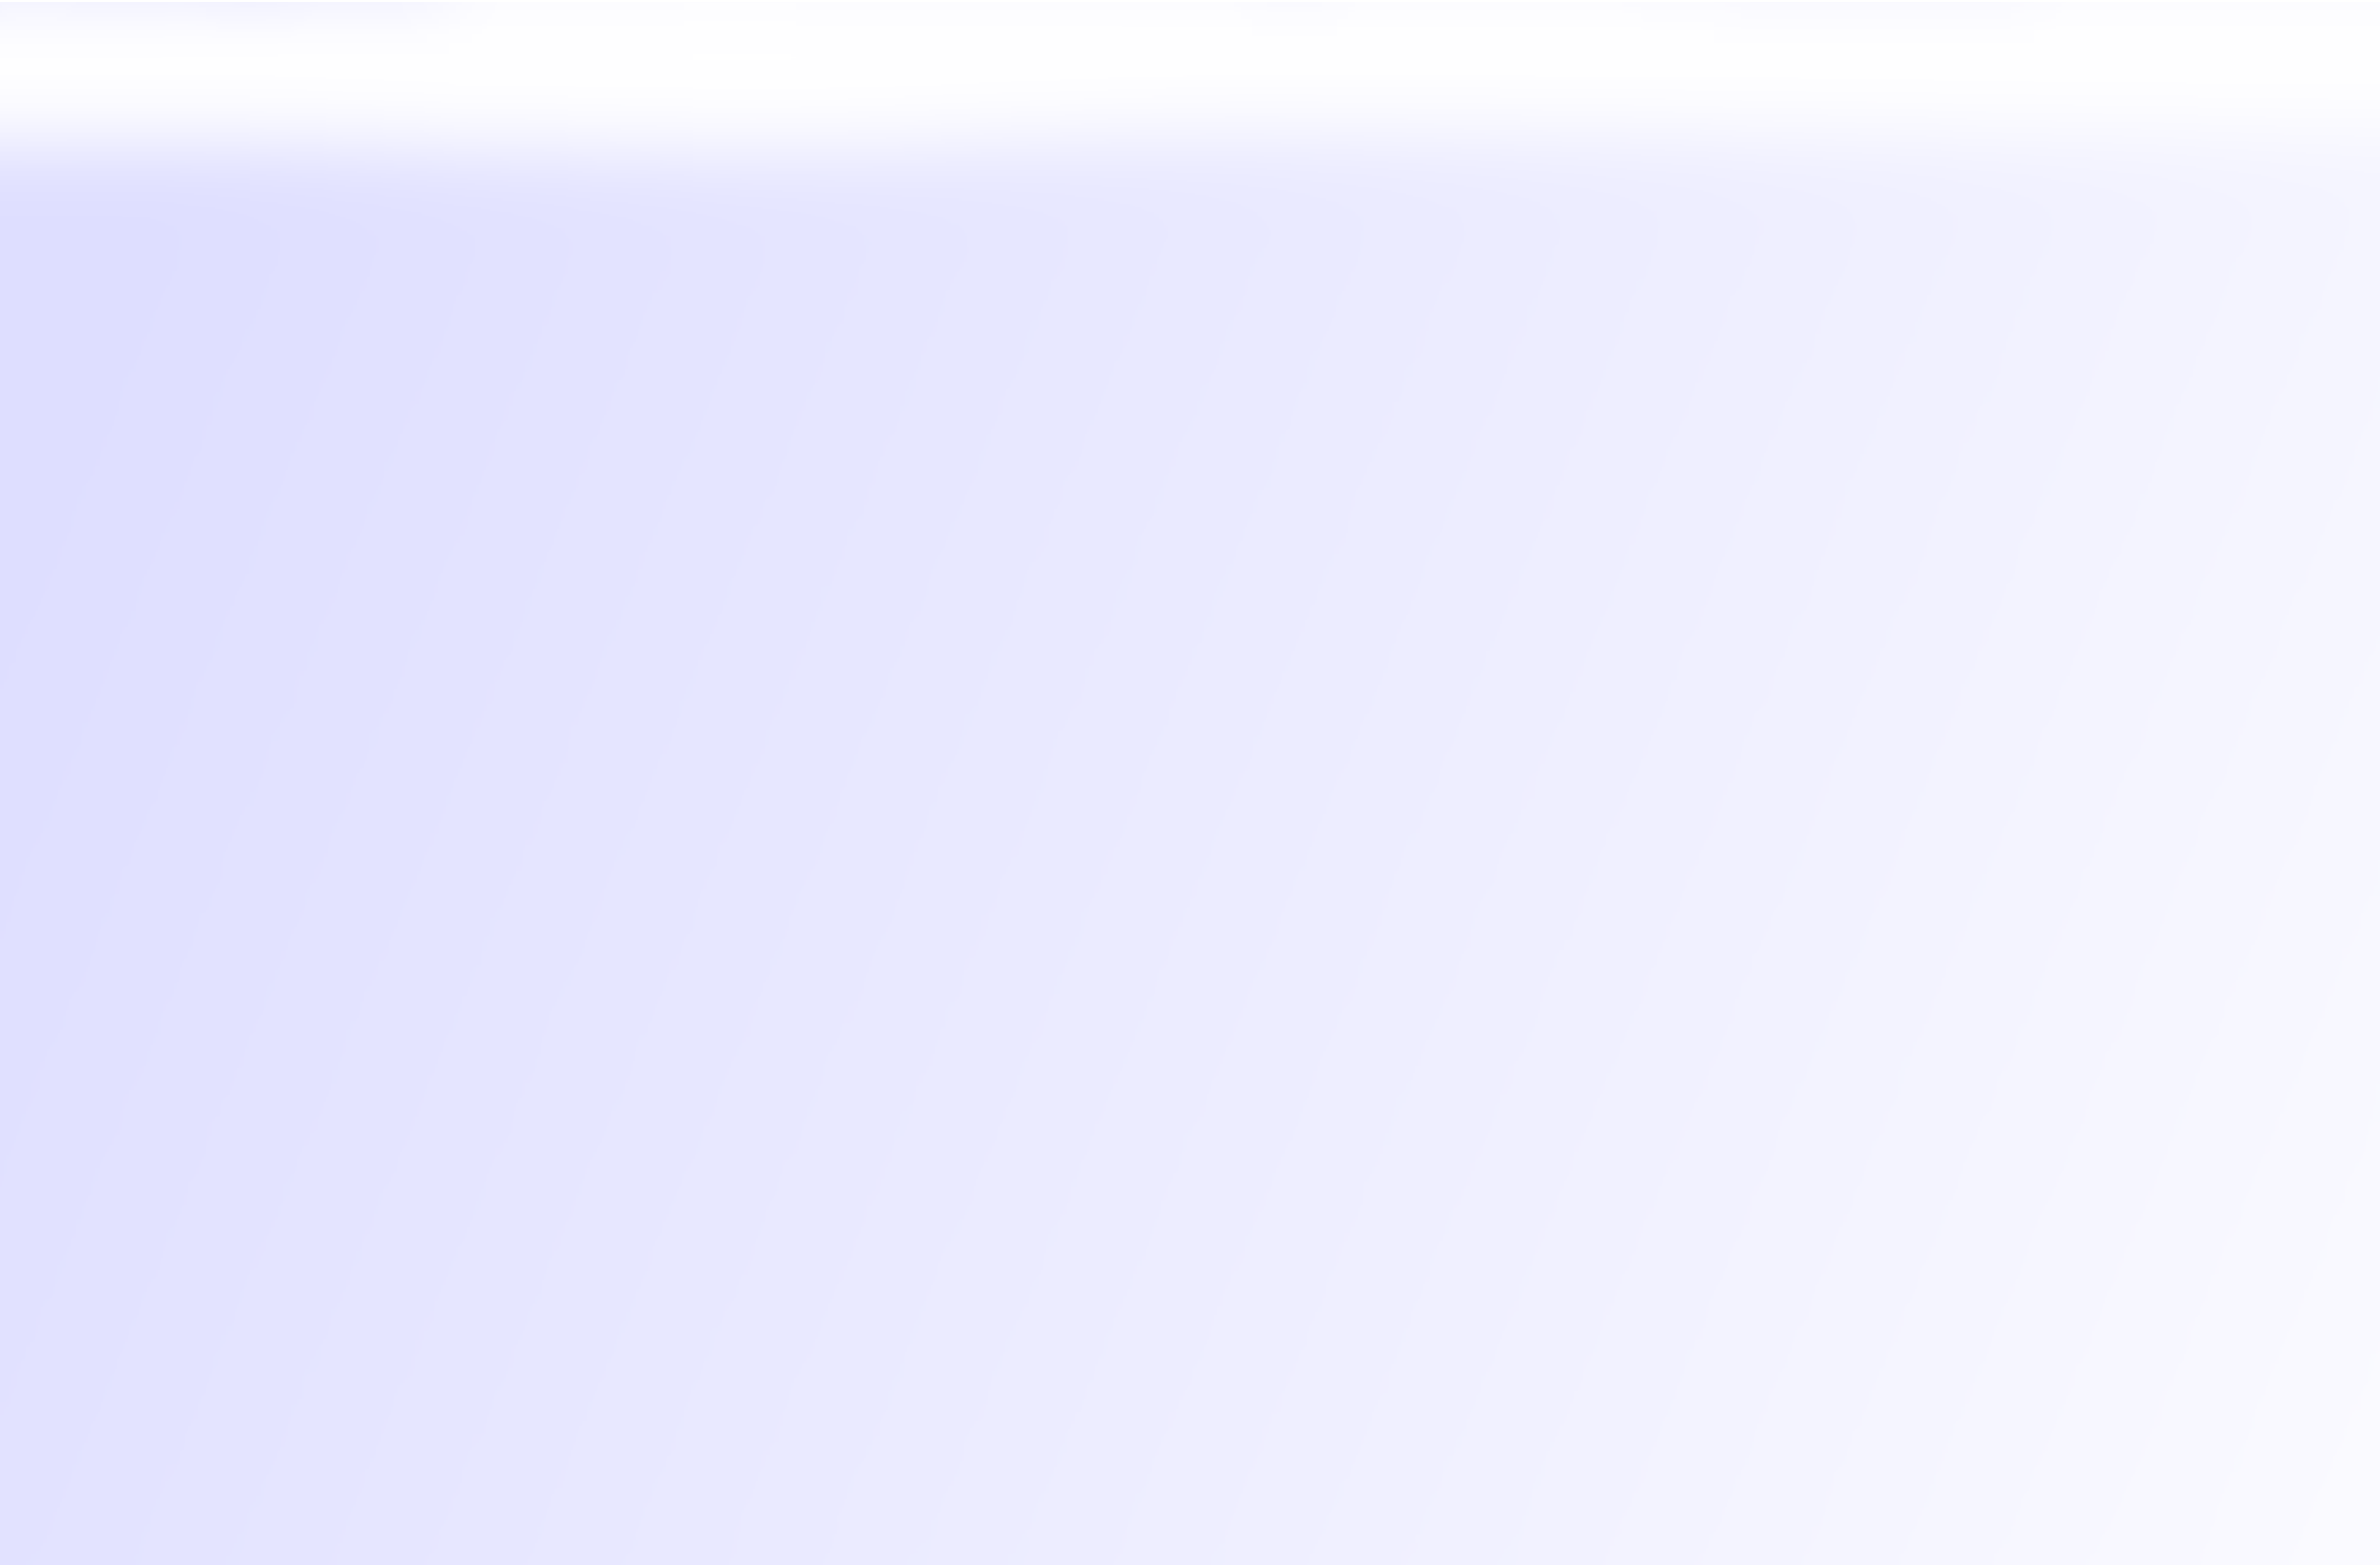
\includegraphics[height=1.1\textheight]{background}};
\end{tikzpicture}
}

\begin{poster}{
grid=false,
columns=5,
borderColor=bordercol, % Border color of content boxes
headerColorOne=headercol1, % Background color for the header in the content boxes (left side)
headerColorTwo=headercol2, % Background color for the header in the content boxes (right side)
headerFontColor=headerfontcol, % Text color for the header text in the content boxes
boxColorOne=boxcolor, % Background color for the content in the content boxes
headershape=roundedright, % Specify the rounded corner in the content box headers
headerfont=\Large\sf\bf, % Font modifiers for the text in the content box headers
textborder=rectangle,
textborder=roundedleft,
background=user,
headerborder=open, % Change to closed for a line under the content box headers
boxshade=plain
}
{}
%
%----------------------------------------------------------------------------------------
%	TITLE AND AUTHOR NAME
%----------------------------------------------------------------------------------------
%
{\sf\bf Runtime comparison solving Gray-Scott equation on different OpenCL devices} % Poster title
{\vspace{0.1em} Michael Quell\\ % Author names
{\smaller michael.quell@yahoo.de}} % Author email addresses
{
\includegraphics[scale=0.37]{TU_Logo}} % University/lab logo

%----------------------------------------------------------------------------------------
%	Abstract
%----------------------------------------------------------------------------------------

\headerbox{Abstract}{name=introduction,span=1,column=0,span=2,row=0}{
An example of a reaction-diffusion equation with chaotic solutions. You can expect patterns to emerge from chaos. A uniformly discretization in space and periodic boundary conditions allows the Fast Fourier Transform to be used, so that when coupled with a suitable time stepping scheme a numerical method that suits the parallelism of OpenCL is obtained. The code was benchmarked on various CPU and GPU devices. Performance results for various problem sizes are shown. Example code can be found at:\\
\url{https://github.com/MichaelQuell/GrayScott-OpenCl}

}


%----------------------------------------------------------------------------------------
%	Solving
%----------------------------------------------------------------------------------------

\headerbox{Solving}{name=conclusion,column=0,span=2,below=introduction}{

The equation is solved using a splitting method, in this case we split the equation into the non linear 
\begin{eqnarray*}
\frac{\partial u}{\partial t}&=& -uv^2 ,\quad \frac{\partial v}{\partial t}=uv^2 \\
\end{eqnarray*}
and the linear part
\begin{eqnarray*}
\frac{\partial u}{\partial t}&=& D_u\Delta u+F(1-u), \\
\frac{\partial v}{\partial t}&=& D_v\Delta v-(F+k)v. \\
 \end{eqnarray*} 
 %\vspace{-5}
 The linear part can be solved exactly in Fourierspace and the non linear could be exactly solved using the Lambert $W$ function, but there is no implementation available for OpenCl, instead fix point iteration is used to solve the implicit midpoint rule. The two parts are combined with Strang splitting\cite{splitting}. The space discretization is equidistant in both axes.

}


%----------------------------------------------------------------------------------------
% Implementation
%----------------------------------------------------------------------------------------

\headerbox{Implementation}{name=methods,column=0,span=2,below=conclusion}{

\begin{enumerate}
\item Initialize the data
\item Time stepping
\begin{enumerate}
\item Call non linear kernel
\item {\bf Compute FFT }\cite{clFFT}
\item Call linear kernel
\item {\bf Compute iFFT }
\item Call non linear kernel
\item Do some output
\end{enumerate}
\item Shut down the program
\end{enumerate}
The linear and non linear kernel operates on each grid point individually and are perfectly suit the parallelism of OpenCl. The most time consuming step is the computation of the FFT and iFFT. Also there is only data transfers from the GPU, when you do some output.
}
%----------------------------------------------------------------------------------------
%	REFERENCES
%----------------------------------------------------------------------------------------

\headerbox{References}{name=references,column=0,span=2,below=methods}{


\smaller % Reduce the font size in this block
\renewcommand{\section}[2]{\vskip 0.05em} % Get rid of the default "References" section title
\nocite{*} % Insert publications even if they are not cited in the poster

\bibliographystyle{unsrt}
\begin{thebibliography}{1}\itemsep=-0.01em
  \setlength{\baselineskip}{1.0em}
  \bibitem{grayscott}
P.~Gray, S.~Scott, Chemical Waves and Instabilities, Clarendon, Oxford, 1990.
\bibitem{splitting}
G. Strang, On the construction and comparison of difference schemes,
SIAM J. Numer.Anal., 5:506-517, 1968.
\bibitem{clFFT}
  clFFT open source library to compute FFT with OpenCl\\
  \url{https://github.com/clMathLibraries/clFFT}
\end{thebibliography}
}

%----------------------------------------------------------------------------------------
%	ACKNOWLEDGEMENTS
%----------------------------------------------------------------------------------------

\headerbox{Acknowledgements}{name=acknowledgements,column=0,below=references,span=2, above=bottom}{

\smaller % Reduce the font size in this block
I would like to thank Benson  {{K}}. Muite  for funding the hardware for the research.
} 

%----------------------------------------------------------------------------------------
%	The Equation
%----------------------------------------------------------------------------------------

\headerbox{The Equation}{name=results1,span=3,column=2,row=0}{ % To reduce this block to 1 column width, remove 'span=2'

The Gray-Scott-equation\cite{grayscott} describes the reaction of 2 chemicals and it is given by 
\vspace{1mm}
\begin{align*}
\frac{\partial u}{\partial t}&= D_u\Delta u-uv^2+F(1-u),\\
\frac{\partial v}{\partial t}&= D_v\Delta v+uv^2-(F+k)v.
\end{align*}
\vspace{-1.75mm}$~$\\
The equation is solved on $[-4\pi,4\pi]^2$ with periodic boundary conditions.
The parameters used in the simulations were $D_u=0.04$, $D_v=0.005$, $F=0.038$ and $k=0.076$. The initial data is a 2-dimensional Gaussian function in both components.

}

%----------------------------------------------------------------------------------------
%	RESULTS 2
%----------------------------------------------------------------------------------------

\headerbox{Results}{name=results2,span=3,column=2,below=results1}{ % To reduce this block to 1 column width, remove 'span=2'

The codes have been tested on following systems, all running Ubuntu 14.04:
\begin{enumerate}[\bf sys 1)]
\item  AMD-A10-5800K $(4\times3.8)$ GHz, APU Radeon HD 7660D, 8Gb ram 
\item  Intel i7-4700MQ $(4\times2.4)$ GHz, GeForce GT 755m, 16Gb ram
\item  AMD FX-8350 $(8\times4.0)$ GHz, Radeon HD 5450, 4Gb ram
%\item Ubuntu 15.10, Intel i7-2600 $(4\times3.4)$ GHz, Radeon HD 7970, 16Gb ram\\
\end{enumerate}
For the performance measuring 500 steps are computed and the Wall-clock  time is used. The problem size started at $32^2$ and is doubled every time, till $4096^2$ is reached for single precision and $2048^2$ for double precision, because of the memory limitation on the GPU's.
%------------------------------------------------

\begin{center}
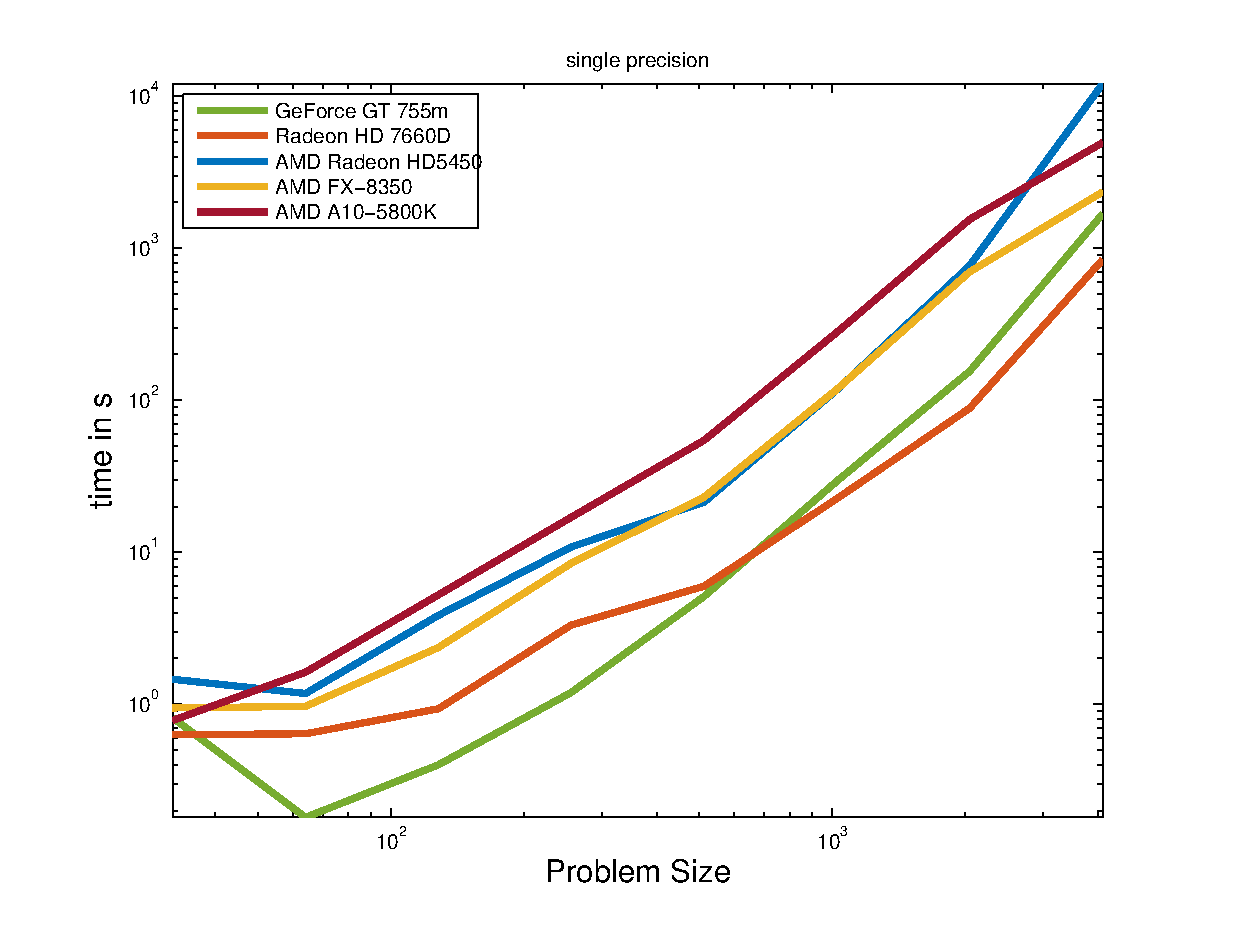
\includegraphics[width=0.49\linewidth]{single2d}
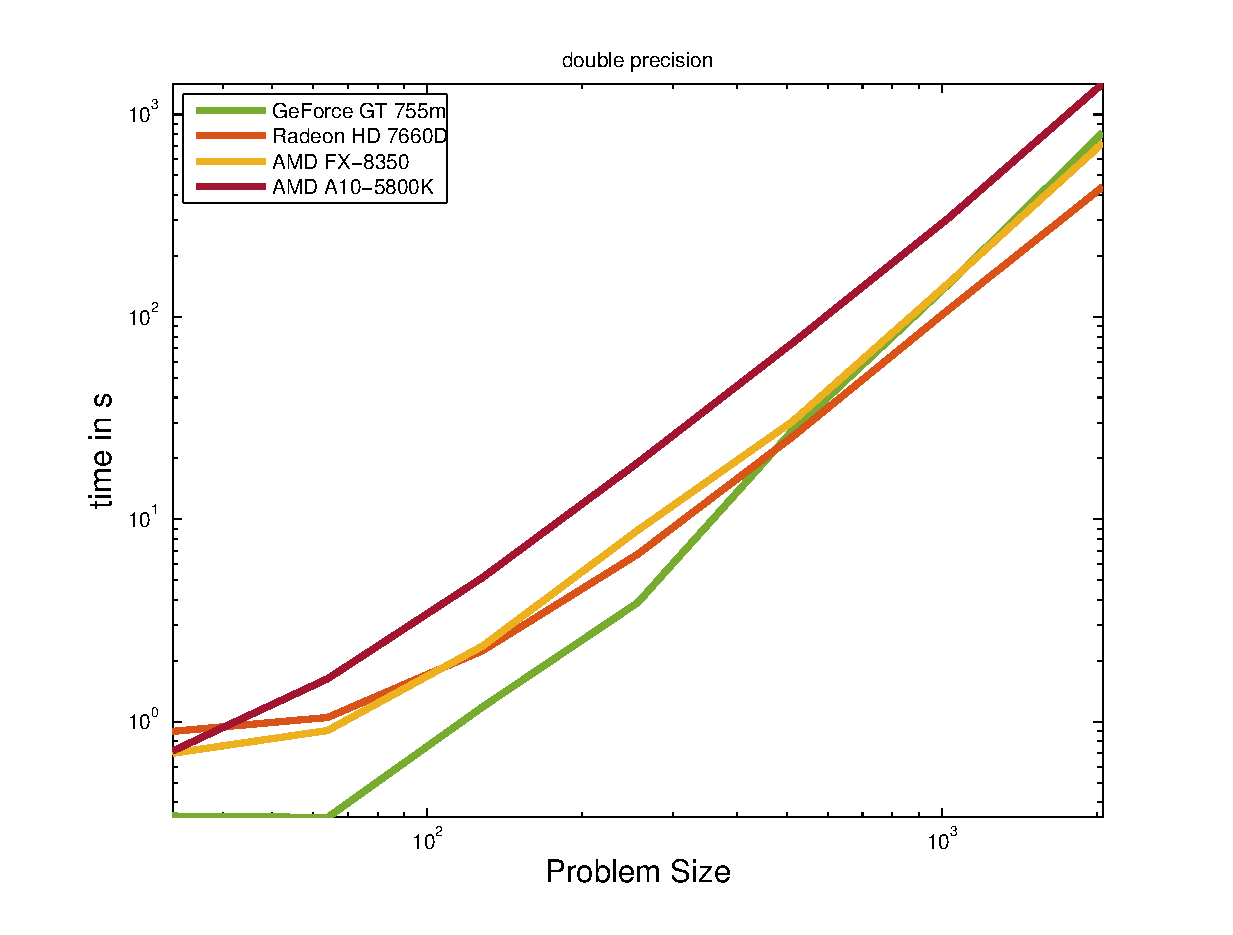
\includegraphics[width=0.49\linewidth]{double2d}
\captionof{figure}{Calculation with single precision (left) and double precision (right)}
\end{center}

%------------------------------------------------



%------------------------------------------------

\begin{center}

\includegraphics[width=0.3\linewidth]{u1}

\includegraphics[width=0.3\linewidth]{u2}

\includegraphics[width=0.3\linewidth]{u3}
\captionof{figure}{Left to right $t=0,500,1500$}

\includegraphics[width=0.3\linewidth]{u4}

\includegraphics[width=0.3\linewidth]{u5}

\includegraphics[width=0.3\linewidth]{u6}
\captionof{figure}{Left to right $t=2250,2500,3000$}
\end{center}

%------------------------------------------------


}


\headerbox{Conclusion}{name=results3,span=3,column=2,below=results2,above=bottom}{ % To reduce this block to 1 column width, remove 'span=2'
The results show that the GPU's outperform the CPU's in single precision, but when computing double precision the performance of the CPU's stays the same, while the GPU's have a significant drop. To compute the equation on larger grids or in 3-dimension, you will, have to face the problem that on GPU's memory is short. One could avoid that by writing a distributed FFT as the other kernels are independent on the problem size. 


}
%----------------------------------------------------------------------------------------

\end{poster}

\end{document}